% !TeX root = ../main.tex
\chapter{测量方案设计}\label{ch:principle}

已有的静电力测量方法均具有较大的不确定性。为了得到更准确、可信的测量结果,需解决一些已有方案中的共有问题,并尽可能减小乃至消除测量中的不确定性,设计出新的测量方案。由于除背吹平衡法以外的方案均在原理上就具有较大不确定度(见\ref{sec:priorArt}节),本章以背吹平衡法作为基础来设计新方案。



\section{背吹平衡法原理分析}\label{sec:principle-backside}


\subsection{受力分析}\label{sec:principle-backside-force}

\begin{figure}[tbh]
\centering
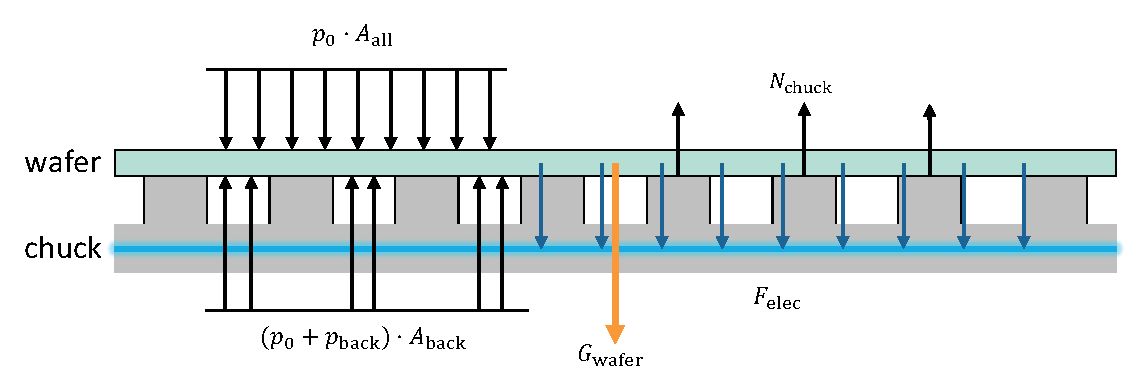
\includegraphics[width=1\linewidth]{principle/force__orig}
\caption{背吹平衡法中晶圆受力分析}
\label{fig:principle-backside-force}
\end{figure}

当静电卡盘处于正常工作状态时,晶圆牢固吸附在静电卡盘表面,其受力情况如图~\ref{fig:principle-backside-force},处于平衡状态,有:
\begin{equation}
\label{eq:principle-backside-force}
(p_{0} + p_{\mathrm{back}}) \cdot A_{\mathrm{back}} + N_{\mathrm{chuck}} = p_0 \cdot A_{\mathrm{all}} + G_{\mathrm{wafer}} + F_{\mathrm{elec}}
\end{equation}
其中:
\begin{itemize}
  \item $p_{0}$ : 环境压强(绝对)
  \item $p_{\mathrm{back}}$  : 背吹压强(相对于$p_{0}$)
  \item $A_{\mathrm{back}}$  : 晶圆背面气压等效作用面积(见\ref{principle-prob-area}节)
  \item $A_{\mathrm{all}}$   : 晶圆总面积
  \item $N_{\mathrm{chuck}}$ : 静电卡盘表面向晶圆提供的总支持力
  \item $G_{\mathrm{wafer}}$ : 晶圆总重力
  \item $F_{\mathrm{elec}}$  : 晶圆所受总静电吸引力
\end{itemize}
当晶圆即将脱附时,有 $N_{\mathrm{chuck}} \to 0$ ;此时 \eqref{eq:principle-backside-force} 可近似为:
\[
(p_{0} + p_{\mathrm{back}}) \cdot A_{\mathrm{back}} = p_0 \cdot A_{\mathrm{all}} + G_{\mathrm{wafer}} + F_{\mathrm{elec}}
\]
即:
\begin{equation}
\label{eq:principle-backside-force-derived}
F_{\mathrm{elec}} = (p_{0} + p_{\mathrm{back}}) \cdot A_{\mathrm{back}} - p_0 \cdot A_{\mathrm{all}} - G_{\mathrm{wafer}}
\end{equation}

虽然分析时将重力与支持力简化等效为集中力,实际上晶圆受到的包括重力与支持力在内的所有力均为分布力。因此,若假设静电力分布足够均匀,上述分析同样适用于晶圆局部。


\subsection{脱附条件}\label{sec:principle-backside-dechuck}

背吹平衡法中,需人为产生并检测晶圆即将脱附至完全脱附的状态,从而间接获得静电力大小。制造脱附条件的基本方法是使背吹压力相对于静电吸引力更大,可通过提高气压、降低电压等方式实现(见\ref{sec:priorArt-backside}节)。检测脱附的基本方法是监测晶圆在脱附时产生变化的物理量,如位移(晶圆挠度)、电极电压/电流、背吹压强/流量等。%TODO:analysis/xref



\clearpage



\section{背吹平衡法中存在的问题}\label{sec:principle-prob}


\subsection{工作环境}\label{sec:principle-prob-env}

静电卡盘常见于工艺腔室中,其内部为真空或绝对压强极低的等离子体(单极型静电卡盘必须在等离子体存在的环境中才能工作)。已有检测方案大多设计为在真空条件、甚至等离子体条件下工作,以复现实际工艺条件。虽然这样可能有助于提高测试结果的准确度,但在真空与等离子体条件下试验存在如下问题:无论等离子存在与否,均需围绕选定的静电卡盘及检测仪器等设计并搭建专真空腔室,系统组成极为复杂,难度与刻蚀机核心部分设计相当。即使已有合适的腔室与配套设备,在开始检测之前,需等待真空泵将腔室抽成真空,时间长达数小时,而一旦需打开腔室进行调整,必须在此之前平衡气压,调整后再花费数小时抽真空,效率极低。此外,当等离子体存在时,晶圆上方大部分空间无法放置任何物体,以避免等离子体受到遮挡或与异物产生相互作用;这对测量系统的设计是过于苛刻的约束条件。


\subsection{间隙与部分脱附}\label{principle-prob-gap}

已有脱附试验(包括但不限于背吹平衡法)中存在一个共有问题:当\emph{检测}到脱附时,晶圆实际已部分脱附,即脱附是一连续变化的过程 %TODO:cite 曹明路
;此时晶圆与卡盘的间隙大于未脱附(正常工作)时,而%TODO:xref bg equations
\begin{comment}
根据,
\end{comment}
静电力随着间隙扩大急剧下降,导致测得的静电力一定小于工作状态静电力,即测量存在较大系统误差。如能设法减小该误差,则可提高测量的准确度。

误差的消除需要更好的脱附检测手段。虽然瞬态过程(如晶圆突然出现明显脱附等)容易检测且不易误判,但此时晶圆并非处于平衡态,且其在微观上可能已大部分脱附,加上检测仪器的响应延迟(精度较高的仪器往往延迟也更大),对系统误差影响极大。为避免瞬态过程带来的系统误差,应维持系统处于准静态或缓变过程中。然后,为了减小部分脱附对检测产生的影响,需快速、准确地判定刚刚开始脱附这一现象;此时间隙未明显扩大,静电力相对于工作状态未出现明显偏差,即减小了系统误差。为此,需选取合适的脱附特征物理量,并设计对应检测手段,改进脱附判定。


\subsection{背吹通道流动}\label{sec:principle-prob-flow}

已有背吹平衡方案均假定晶圆背面受均匀压强作用,但未论证该假设的合理性:背吹通道中存在的流动是否会影响晶圆背面受力情况?若有,则测量方案的准确度可能会受到影响。因此,有必要分析晶圆背面的流动情况。

\subsubsection{建立CFD模型}\label{sec:principle-prob-flow-cfd-setup}

为了方便后续仿真工作的开展,此处选择Comsol作为仿真软件;先搭建简化模型,做出基本判断,再根据后续试验需要,进一步添加细节,提高仿真准确度。

\begin{figure}[tbh]
\centering
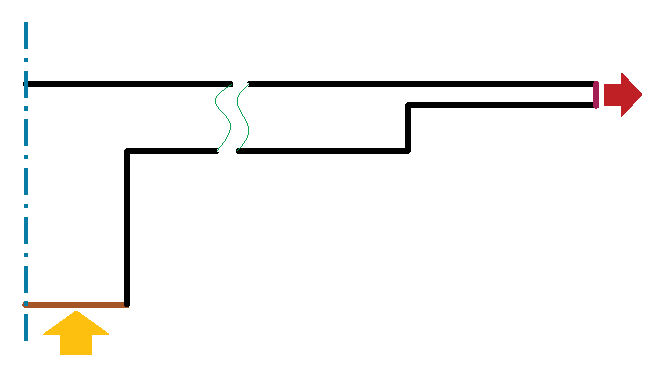
\includegraphics[width=0.72\linewidth]{principle/cfd__setup}
\caption{晶圆背面流动CFD建模示意}
\label{fig:principle-flow-cfd-setup}
\end{figure}

由待测静电卡盘\footnote{具体参数见\ref{sec:rig-overall}节。}背吹通道特点知,流动主要为平板间层流,因此选用层流模块(\bverb|spf|)求解。几何模型选用二维轴对称(2D Axisymmetric,即纯旋转体),流道截面如图~\ref{fig:principle-flow-cfd-setup}\footnotemark{};在正中间设一圆柱形进气口,直径\SI{1}{\mm},固定其压力为\SI{2}{\kPa}表压;在边缘处用均匀圆环形狭缝来等效晶圆与陶瓷介电层的接触密封,外侧设为出口,固定为大气压。

\footnotetext{此处流道宽度由陶瓷介电层表面的凸台高度决定,但为了简化分析起见,暂时忽略凸台影响。}

由于目前对接触密封的了解尚少,无法准确估计等效狭缝宽度,因此设定参数扫描,求解当狭缝宽度为$\SIrange{1}{0.1}{\micro\meter}$(\bverb|10^{range(0,-1/2,-1)}[um]|)时的流动情况。

\subsubsection{CFD仿真结果}\label{sec:principle-prob-flow-cfd-result}

当狭缝宽度改变时,速度场变化不大,最大速度均出现在进口附近,之后速度迅速衰减至稳定,如图~\ref{fig:principle-flow-cfd-result-vel} 。

%TODO:动量呢?

在入口处对$v_z\ \rho$取面积分,得到质量流量如表\ref{tab:principle-flow-cfd-result-flow}。单位\si{\mg\per\minute}大致与sccm相当,即质量流量在狭缝宽\SI{1}{\micro\meter}时,仍低于1 sccm;狭缝变窄时,流量得非常快。这说明只要密封处的实际表面粗糙度足够低,接触足够紧密,则气体泄漏几乎可忽略不计;若安装流量计,则应选取较小量程的型号(一般为10 sccm)。

沿模型上边界(即晶圆下表面)绘制压强 -- 半径曲线,如图~\ref{fig:principle-flow-cfd-result-pressure} ,发现在流道中段压降满足$\Delta p \propto \log{r}$。 %TODO:derive by hand
当狭缝宽\SI{1}{\micro\meter}时,在中段存在明显压降(约\SI{0.6}{\kPa}),显然\textbf{不能忽略};但当狭缝更窄时,压降迅速衰减,当狭缝宽\SI{0.3}{\micro\meter}时已可忽略。当然,这是假定只有卡盘中央有一个气孔的时候的情形,而实际的静电卡盘为了控制温度分布均匀,在整个表面多处分布气孔,可使压强分布更均匀。即便如此,在处理实验数据时,应小心验证压强分布(可进一步构建三维流道模型以得到更准确的仿真数据),不能直接认为晶圆受均匀气压作用。

\begin{table*}[thbp]
\centering
\caption[CFD结果:质量流量]{CFD仿真结果:进口处质量流量}
\label{tab:principle-flow-cfd-result-flow}
\begin{tabular}{SS}
  \toprule[1.5pt]
  狭缝宽度/\si{\mm}  &  质量流量/\si{\mg\per\minute}  \\
  \midrule[1pt]
  \num{1.000}  &  \num{2.183e-1}  \\
  \num{0.316}  &  \num{9.628e-3}  \\
  \num{0.100}  &  \num{3.079e-4}  \\
  \bottomrule[1.5pt]
\end{tabular}
\end{table*}

\begin{figure}[hbp]
\centering
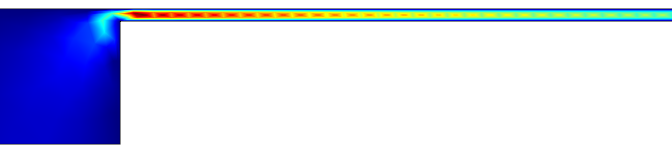
\includegraphics[width=0.72\linewidth]{principle/cfd__vel.png}
\caption[CFD结果:速度场]{CFD仿真结果:进口附近速度场}
\label{fig:principle-flow-cfd-result-vel}
\end{figure}

\begin{figure}[hbp]
\centering
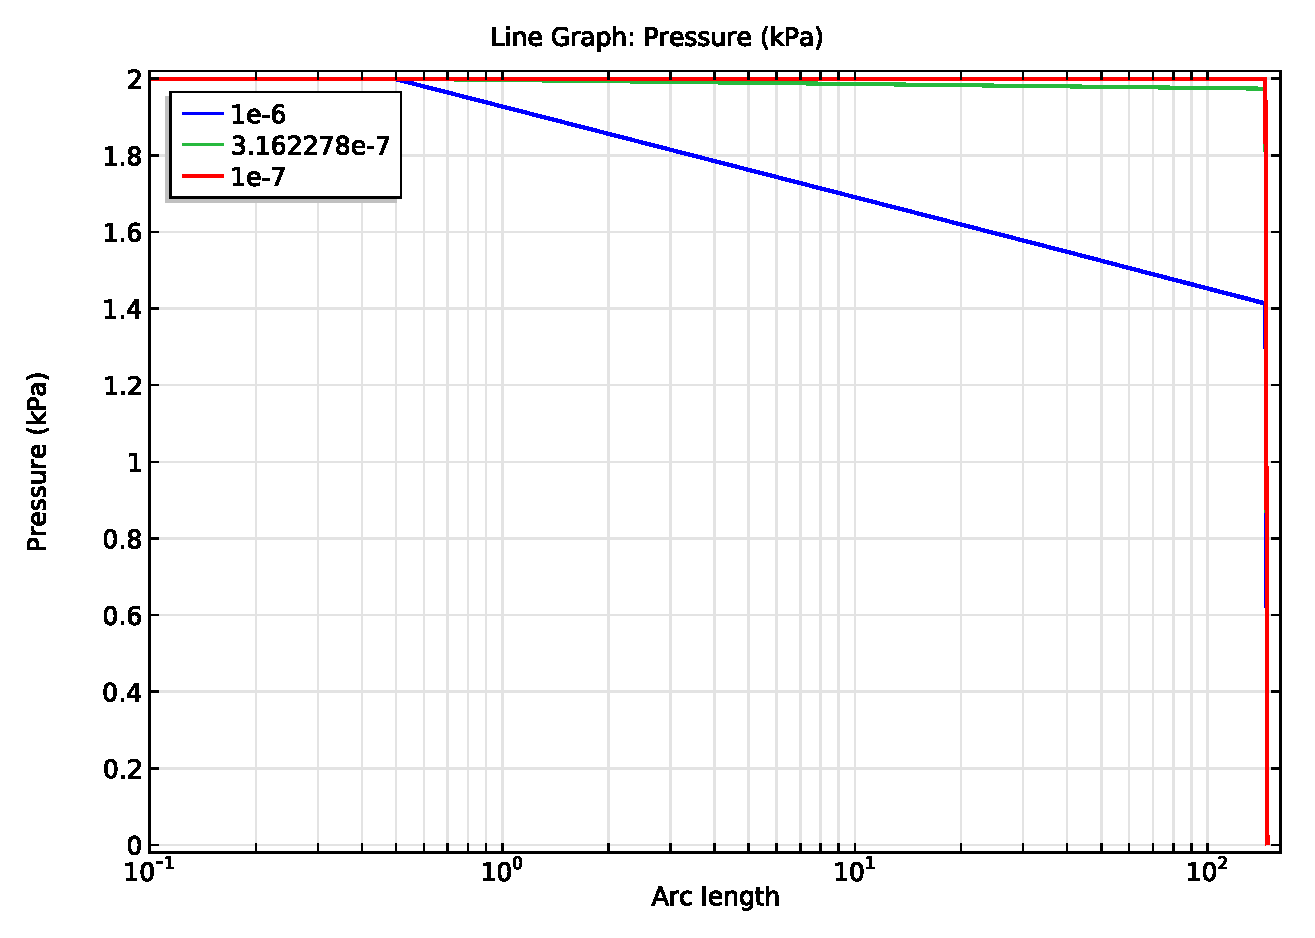
\includegraphics[width=1\linewidth]{principle/cfd__pressure}
\caption[CFD结果:压力分布]{CFD仿真结果:压力沿径向分布}
\label{fig:principle-flow-cfd-result-pressure}
\end{figure}


\clearpage


\subsection{压强等效作用面积}\label{principle-prob-area}

\eqref{eq:principle-backside-force}式中,晶圆背面气压等效作用面积(即$A_{\mathrm{back}}$)是未知量。
%TODO:cite nagoya
由于陶瓷介电层上的凸台高度较低(约\SI{10}{\micro\meter})与晶圆背面接触情况不明,尚不能直接断言$A_{\mathrm{back}}$等于晶圆背面所有未与陶瓷层凸台/边缘接触部分的面积。由于此处无法用普通CFD求解,需要设计额外的标定步骤,测出$A_{\mathrm{back}}$数值。



\section{改进方案设计}\label{principle-soln}


\subsection{工作环境}\label{principle-soln-env}

由\ref{sec:principle-prob-env}节中讨论,真空与等离子体环境均不利于检测系统的设计、实现与使用,因此改进方案为在大气环境下使用设计,并可在不改变主要原理的条件下,经过尽可能少的修改,移植到真空腔室中;等离子体环境不予考虑。


\subsection{引入微力探头判定脱附}\label{principle-soln-ruby}

\begin{figure}[tbhp]
\centering
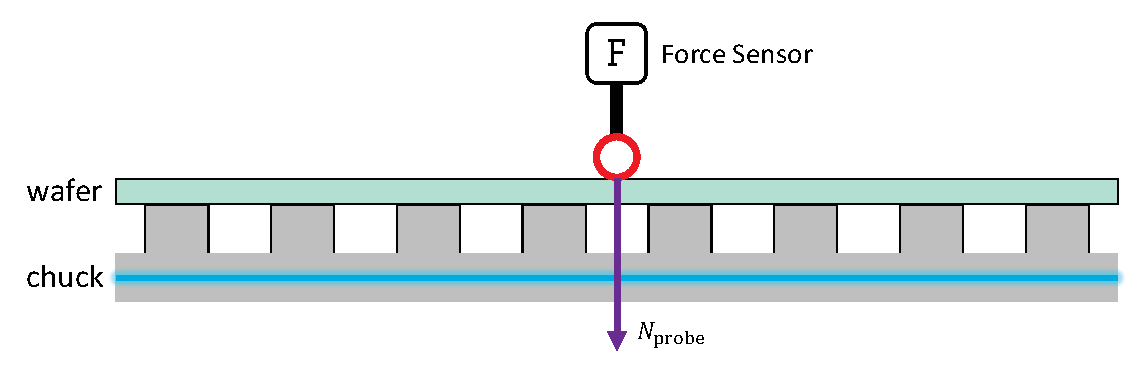
\includegraphics[width=1\linewidth]{principle/soln__ruby__sch}
\caption{微力探头原理示意}
\label{fig:principle-soln-ruby-sch}
\end{figure}

考虑\ref{sec:principle-backside-force}节中的受力平衡关系。虽然在即将脱附时,$N_{\mathrm{chuck}} \to 0$,但此时存在\ref{principle-prob-gap}节中阐述的间隙扩大问题。如果希望抑制间隙扩大,则必须向晶圆施加一个向下的力$N'$。注意即使晶圆在即将脱附时,其在$N'$作用下仍处于平衡状态,且力平衡方程变为:
\begin{equation}
\label{eq:principle-soln-ruby-force}
(p_{0} + p_{\mathrm{back}}) \cdot A_{\mathrm{back}} + N_{\mathrm{chuck}} = p_0 \cdot A_{\mathrm{all}} + G_{\mathrm{wafer}} + F_{\mathrm{elec}} + \mathbf{N'}
\end{equation}
若$N'$大小可测量,则可将其作为脱附特征物理量,准确判定部分脱附。据此设计微力探头,如图~\ref{fig:principle-soln-ruby-sch},其组成为一单轴微力传感器以及连接在其上的标准三坐标测量机红宝石探头(图中以红色圆形表示,实际为球体)。晶圆吸附后,使红宝石探头与已吸附的晶圆表面接触,探头方向垂直于晶圆表面,则由牛顿第三定律,传感器受到的压缩力和探头施加在晶圆上的支持力$N_{\mathrm{probe}}$大小相等\footnotemark{};若采取措施确保此时$N_{\mathrm{probe}} \ll F_{\mathrm{elec}}$,则可认为$N_{\mathrm{probe}} \approx 0$。逐渐增加背吹气压,直至晶圆脱附这一过程中,$N_{\mathrm{chuck}} \to 0$,并逐渐转由探头向晶圆提供支持力,即$N_{\mathrm{probe}}$明显增加,可作为判定晶圆开始脱附的根据。由于传感器自身具有一定弹性(在量程范围内可等效为一理想弹簧),晶圆在与探头接触的一点仍有一定挠度,但由胡克定律$F = k x$知,该点挠度可由测得的$N_{\mathrm{probe}}$和传感器刚度$k$计算出,并且对于给定传感器,$k$已知,而$N_{\mathrm{probe}}$可人为地在传感器量程内选取有效取值区间,因此在判定脱附时,该挠度也处于一个确定的取值区间内,即晶圆与卡盘的间隙得到了控制。

\footnotetext{即为上文$N'$;另外,下文中不再区分这一对反作用力,仅用$N_{\mathrm{probe}}$表示其大小。}


\subsection{晶圆自重平衡法求压强等效面积}\label{sec:principle-soln-gravity}

\begin{figure}[tbhp]
\centering
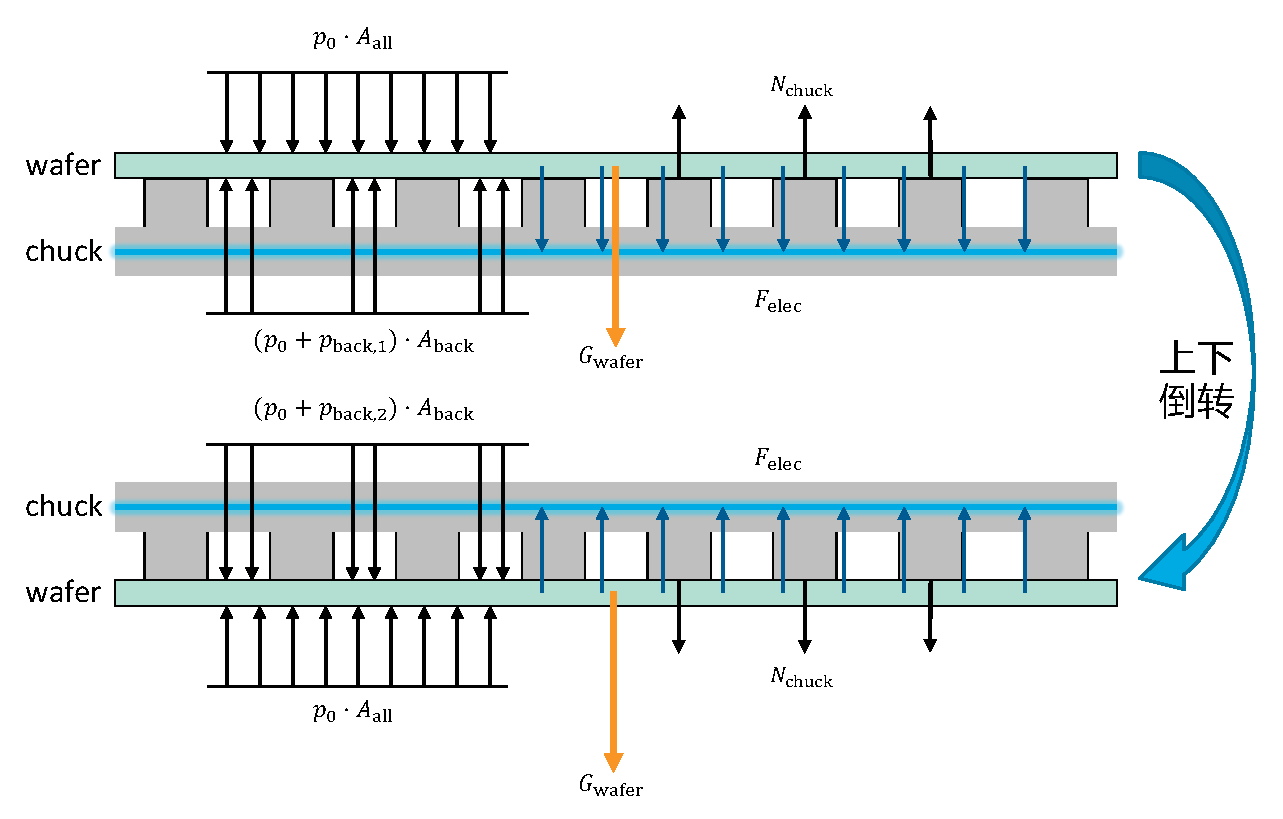
\includegraphics[width=1\linewidth]{principle/area__gravity__sch}
\caption{晶圆自重平衡法求压强等效作用面积示意}
\label{fig:principle-area-gravity-sch}
\end{figure}

建立一个固连在静电卡盘上的坐标系,注意到在晶圆受力平衡关系中,除重力以外,其他力相对于该坐标系的方向均固定,而重力方向随着静电卡盘姿态改变而改变。若将静电卡盘上下倒转\ang{180},则相对于静电卡盘坐标系,只有晶圆受到的重力方向反转。据此可求出压强等效面积:分别在试验台正放和倒放两种状态下,加相同电压,完成背吹平衡试验,得到即将脱附时的背吹压强分别为$p_{\mathrm{back},1}$和$p_{\mathrm{back},2}$(可通过多次测量取平均值的方法来减小随机误差)。根据受力平衡关系有:
\begin{equation}
\label{eq:principle-area-gravity-orig}
\begin{aligned}
(p_{0} + p_{\mathrm{back},1}) \cdot A_{\mathrm{back}} & = p_0 \cdot A_{\mathrm{all}} + G_{\mathrm{wafer}} + F_{\mathrm{elec}} \\
(p_{0} + p_{\mathrm{back},2}) \cdot A_{\mathrm{back}} & = p_0 \cdot A_{\mathrm{all}} - G_{\mathrm{wafer}} + F_{\mathrm{elec}}
\end{aligned}
\end{equation}
两式相减:
\[
(p_{\mathrm{back},1} - p_{\mathrm{back},2}) \cdot A_{\mathrm{back}} = 2 G_{\mathrm{wafer}}
\]
即:
\begin{equation}
\label{eq:principle-area-gravity-derived}
A_{\mathrm{back}} = \frac{2 G_{\mathrm{wafer}}}{p_{\mathrm{back},1} - p_{\mathrm{back},2}}
\end{equation}
即求得$A_{\mathrm{back}}$数值。需要注意的是,$A_{\mathrm{back}}$可能与所加电压、晶圆材料、厚度等各种参数相关,可改变条件,多次试验,得出$A_{\mathrm{back}}$对各参数的敏感度。



\section{本章小结}\label{sec:principle-summary}

本章首先分析了原有背吹平衡法检测静电力的工作原理,指出了其中存在的影响测量准确性的因素,包括晶圆部分脱附、晶圆与静电卡盘间存在的间隙扩大、背吹通道流动对晶圆背面压强分布的影响、以及压强等效作用面积等,进而针对其中最主要的部分脱附、间隙、以及压强等效作用面积问题,提出微力探头、自重平衡两种措施作为改进方案,并阐明了其减小原有方案中误差的原理。
